\section{Proposed Research and Methods}
\label{subsec:challenges}
\label{sec:proposed}

%\begin{enumerate}
%\item Re-factoring of the data
%  \begin{itemize}
%  \item What kind of reorganization would work when?
%  \item Would it take too much time and resources + memory and how can we
%    manage the cost of the reorganization
%  \item Will the users loose too much value from the data during refactoring
%    and how can we control/bound this loss of value
%  \end{itemize}
%\item Quality of Service
%  \begin{itemize}
%  \item Can we make any guarantees in a scalable decentralized system?
%  \item What quality of service metrics can be make guarantees on in a scalable
%    way?
%  \item What kind of error rates will we have in our estimation and what error
%    rates are acceptable?
%  \item How much will the qos scheduler, admission control, manager cost in
%    terms of resources and time
%  \item How do we make the scheduler scalable with the size of the system?
%  \end{itemize}
%\item Discovery and naming
%  \begin{itemize}
%  \item Which data block and what quality/type do we respond to a query
%    with?
%  \item How will we scale a fully distributed storage system's metadata
%    management
%  \item Can we accelerate the discovery process with the addition of an
%    application/user level metadata store that tracks where data was
%    originally written and how was it structured?
%  \item Can we provide time estimates for read/write calls in the presence of
%    an unbounded discovery system? If not how do we bound the discovery time?
%  \item Time cost of discovery vs time cost of actually reading the data
%    (latency vs bandwidth essentially)
%  \end{itemize}
%\item Migration
%  \begin{itemize}
%  \item Can we do scalable migration without making the discovery process
%    unbounded
%  \item What are the parameters and input for migration
%  \item Can we use the additional application level knowledge of data to purge
%    portions of the data from storage without making the data too much less
%    valuable?
%  \item With so many objects and no centralized directory how do we know what
%    is actually in the storage to be purged?
%  \item How do purge in a way that doesn't require a central authority,
%    doesn't interfere with other I/O and isn't bottlenecked by some sort of
%    global consistency
%  \end{itemize}
%\end{enumerate}


%Our research into the storage system and middle ware layers must address
%many of these challenges including
% \begin{enumerate}
% \item How do we describe the user intentions at the API layer and have this
%   communicated down to the middle-ware and storage layers?
% \item How do we allow users to define their user defined compression
%   techniques and have this data read back from the storage system layers?
%   Where do we execute the decompression techniques 
% \item How do we evaluate the tradeoffs at runtime to guide data placement,
%   including the movement of data across the network, across the different
%   storage tiers? (data movement and quality tradeoff)
% \item Can we use different forms of learning techniques as daemons on the
%   system to perform data migration from one storage tier to another? For
%   example, if we see that a user is looking at one time slice after another
%   for a certain object in their dataset which is in the slower tiers of the
%   hierarchy, do we automatically propane up the data which has not been
%   requested in the hope that this will be requested data? (prediction and
%   prefetching, user defined compression on movement)
% \item Can we understand the true need of campaign storage and understand the
%   possible impact of the campaign storage if we run a hadoop-like
%   file-system instead of a lustre/gpfs file system? (additional layers)
% \item Can we limit the amount of data duplication? Data space is going to be
%   very constrained on the exascale system so we must ensure that minimal
%   copies are made of data, and when data is duplicated, they are removed
%   through a garbage collection routine. (space management)
% \item Can we build a model to give us the time estimates during the reading
%   and writing phases, so that rules can be in place from the user
%   perspective to make adaptive decisions. For example, if the file system
%   says that reading will take 3 months, users can they place in rules to
%   then read in a subset of data, and they can understand which data can be
%   read quickly and which pieces will take more time. (estimation)
% \item Can we understand how to place code in the system which will allow
%   data-regeneration to take place. (regeneration)
% \item How does the storage system do a better job in managing request from
%   all of the users on a LCF than today? We realize that today users who have
%   a better middlware system can often lock other users from getting high
%   performance when they are running. If we have the concept of currency
%   which is eventually used in the same extent as node-hours, then users will
%   have to be able to think about how much storage and how much bandwidth
%   they can choose. One question that needs to be understood is if there are
%   times when the system sees that there are very few storage system
%   resources being used, then the lucky users can get the bandwidth cheaper
%   than at times of heavy usage. How can we enforce this? (Fairness)
% \item How do we manage all of the metdata not only from the principle
%   objects, but from the sub-objects? How well will this scale when we have
%   users who can potentially create billions of objects from their
%   simulation? (scalability and discovery)

%\paragraph{Deliverables and artifacts}
%
%\begin{enumerate}
%\item Add plug-in architecture to Sirocco to support selective data compression
%\item Add specific tier destinations command to Sirocco (assuming that the caching mechansism cannot achieve the desired effects).
%\item Develop profiling system to determine how a data set is used during preparation runs prior to a capability run to determine how to optimize data placement for capability run analytics.
%
%\end{enumerate}
%
%{\bf \color{red}we need to condense these challenges into a few basic principles - 4 at most - SAK}

We propose to overcome these challenges by pioneering a new {\bf
knowledge-centric approach} to a dynamic storage system and I/O layer which
takes into account user prioritization and utility to optimize the SSIO layer.
The approach is based on two underlying principles:

\underline{Principle 1:} {\bf A knowledge-centric system design} that allows user knowledge  to
define data policies. Today SSIO layers are written in a
stove-pipe fashion, and quite often do not allow optimizations to take place.
We propose to re-design the layers in a highly integrated fashion where users
will place their intentions into the system and actions will statically and dynamically
take place to optimize for both the system and for individual
requests.

\underline{Principle 2}: {\bf Predictable performance and quality of data in the SSIO layers} needs to be
established so science can be done on the exascale systems in a more efficient manner. Without
predictable performance, not only can the runs be slowed down because of contentions \cite{liu_hotstorage}, 
but also it affects key science decisions, e.g., how much data reduction should be performed.
It is clear that if a run is expected to be slow, an aggresive data reduction needs to be performed
so that science can be done in a timely fashion, which has been reflected in the XGC run (\S~\ref{sec:introduction})
that the PI recently participated.

We aim to alleviate the need for the ``magic'' and ``tricks''
that are currently required to optimize application I/O performance
on today's file systems. To accomplish this, we will provide a systematic
approach for describing intentions and other knowledge from {\it user}
space, as well as allow performance estimations and guarantees 
from the underlyingree storage.
%For example, ADIOS contains most of the ``best practices'' for I/O optimizations for
%   each file system, and as users place more knowledge into ADIOS, ADIOS
%   can make optimizations.
By capturing user intentions and acting upon them in the middleware, we
free the user from polluting application code with system specific
optimizations which may provide better performance in the short term,
but are detrimental to the long-term maintainability of applications, and
are more sensitive to changes to system configuration. We have successfully
employed this strategy of separation of concerns in ADIOS, and believe that
it will become increasingly important because saving all data may not be possible, and
users want the ability to describe and prioritize different chunks of data. 
Our research is aimed to allow users to provide simple descriptions of their data,
which further allows the middleware and storage to optimize application I/O performance.

Additionally we recognize that HPC applications exhibit a set
of common I/O patterns \cite{lofstead2011six,polte2009and,tian2011edo,tian2012system}.
Throughout our project we will continuously focus on creating research artifacts 
which can optimize these I/O patterns on current and
exascale systems. One key focus is Checkpoint/Restart (C/R), leveraging NVRAM to accelerate
checkpoint and data retrieval. 
The migration and purging of this will be optimized by SIRUS using the utility function of 
the C/R data so that this can be stored for short periods of time, and then purged. 



%\underline{Principle 3:} {\bf Users goals define data policies} In a data-centric SSIO system. 
%We introduce data-driven SSIO optimizations by
%enabling users to define data manipulations (re-organizations) at a high level
%and then we express policy goals by associating intentions (hints) with data;
%e.g. ``this data at this level should be accessible within 100 seconds in the
%next three months.'' These high level specifications of desired results will be
%used in our system for data migration and eviction policies.

\subsection{Data Description}
In order for the middleware and storage layer to make decisions
that are appropriate given the user's intentions, data must be
described in a way that communicates these intentions to
the system. In this project, we label the smallest unit of data
saved in the storage system as a \textit{chunk}.  A chunk consists of not only
raw data, but also metadata that expresses additional
knowledge about that data.
A user space variable, such as \textit{temperature}, may
consist of a collection of chunks, possibly with different accuracy or
resolution, and with each chunk representing
a different portion of the variable.
A key advantage of having attributes at this lowest level is that it allows data
semantics, user intentions, QoS requirements, and the relationship between user
data to be readily captured and embedded with the raw data so that these
smallest pieces can each be managed independently or collectively, depending on
the need. As an example, retrieving 3D field data generated from a simulation
and then visualizing it requires the coordinates and connectivity variables be
accessed simultaneously and with low latency to achieve a good user experience.
Managing data at this low level
bridges the semantics gap between applications, middleware, and storage
systems and allows the system to understand user-level data, execute QoS
requirements and policies, and optimize application and system performance.

%The new APIs will enable the bridge by specifying selectable
%performance/quality/- cost tradeoffs from both the application and system
%perspectives based upon the user guided rules/policy and runtime system
%monitoring status. It allows the middleware to make best possible decisions
%from the feedback of storage system knowledge, such that it will embed user
%intentions and the available system storage.  We want the system to give the
%users a certain amount of currency in terms of bandwidth, storage space on
%each level, and latency expectations. These notions will be fuzzy but they
%will allow the user to make ad-hoc decisions to figure out what needs to be
%saved.

The data description may be stored with the individual chunks or within a
separate metadata service or both to aid QoS requirements. It would contain
conventional attributes such as data type, size, dimensionality, and the
relationship to other data. In particular, the relationship to other chunks can
be captured by including \textit{typed links} each representing a different
relationship type.  In this project, a key metric stored as a metadata
attribute is \textit{data utility}.  It enables QoS scheduling, data placement
decisions, data lifetime decisions, and captures the chunk priority. It is
our belief that exascale science will require users to prioritize a small set
of chunks to be saved on higher-level capacity-limited storage to avoid the
slow access to large-capacity lower-level storage, such as tape.  We propose a
new technique, described by a utility function provided by a user, where chunks
can be cast into multiple data buckets and each bucket can be prioritized
differently according to its utility value.  Once this is done, the middleware
system will construct the data description and re-organize and place data to
achieve the desired QoS goals and policies.

A key insight in this proposed project has been the increased interaction of
the application with the storage system.
The user would like to have the ability to obtain information about, and even
negotiate with the system to determin what
level of Quality of Service is possible given
a prospective set of I/O operations and current state of the system, so that
they can then make decisions about what data to access when.
%for example is less than what they desire and will then place in a certain set
%of rules which the system can make autonomic decisions to help decide what
%should be done.
Towards this end, we propose to
address the QoS requirements by providing the application with mechanisms to
specify the quality of I/O service, interrogate the storage system, and react
to the responses. Guided by our past work we propose to explore the design of
mechanisms for this purpose. 

Our research will address the following questions:
1) How can users interact with the storage system efficiently?
2) How can users express their intentions into actionable items which can take place in the middleware and/or storage layer?
3) How can users annotate data with a utility metric?

\paragraph{State of the art:}
Our current data annotation techniques demonstrated in
ADIOS~\cite{lofstead:2009:adaptible} implement a binary-packed data format that
allows data characteristics such as min, max and index to be wrapped around
data chunks. A direct benefit is that each data chunk can be operated upon
independently and I/O concurrency can be maximized. We will build upon this
capability and further augment the format to express data utility.
Recently
DAMSEL~\cite{damsel} has provided a rich metadata representation and management
layer that captures the relationship between data blocks for scientific
applications.  This allows application data to be mapped to storage system
efficiently, without overburdening users with the management of complex data models, such
as AMR, from the user space. Despite these efforts, the aspect of data importance has yet to be 
explored, and we believe it will be vital for exascale storage solutions.
{\color{red}\bf there must be other work in this area, and we need to get more
references}

\paragraph{Proposed research approach:} 
We will design and develop new techniques for data management, description,
and access that allow users to describe the data utility based on their
expectations. This can be done by allowing users to plug in functions that
provide data-specific functionality to the middleware and storage system.
These functions may be executed by the system to
calculate the utility value for each chunk, handle custom compression
and decompression, and perform other data-specific services, thus allowing
the system to more effectively manage data placement and retrieval.
%
%We will design an updated I/O API that will expand on the current POSIX I/O
%semantics by adding new information to the I/O request.

We will explore the space of application level hints that can be provided easily
to the storage system. These hints will enable the storage system to make the
most appropriate optimization decisions for this user in the context of the
multi-user environment rather than trying to rely on a one-size-fits-all
approach. In particular, we expect the application to provide hints on the
length of time before the output data is persistent and visible to users and
the expected data lifetime for output sets. For read calls we envision
hints that provide latency and precision requirements. Additional hints will
also be investigated. 

We will also develop a new type of querying system that allows an application
to ask the storage system about completion timing information. The response
would be an estimated time for the described operation. We will explore
how these query functions can be integrated into common applications with
minimal code disruptions and the set of policies that applications can use to
respond to this new information. We will also explore how applications can
query the storage system to gain insights on available space in different tiers
and how applications can tailor their output data to most effectively use the available space.
Finally we will study the use of an external data annotation system that can
provide information to the storage system without requiring the application to
be recompiled. 

%
From an application level, we will explore these techniques through our ADIOS
framework using many of the applications to which we have access, including
XGC1, GTC, and SPECFM3D. We will investigate: 1) what hints the users can give
the system, 2) how the users can replace much of their
application specific code with
``system level code'' through the use of these hints.  We will design an API
that will be integrated with the storage layer to give time estimations so that
users can decide which data priorities will be written and read. The utility
value for each chunk will be used to sort the chunks into prioritized bins.
Chunks in a particular bin will be assigned an appropriate storage
 tier and lifetime, which can be decided by the user through the API.
For example: in Figure~\ref{fig:ssio-bucket} we have data that
comes from the XGC1 code.  The user can pick a data-refactoring scheme (see
Sec~\ref{sec:data-refactor}) which will bucket the particle data into 4
prioritization levels.  The user can then pick a data utility, such as 3 months
for the highest priority items and 12 months for the lowest priority data.
The user will then call a function, provided by the API, that allows them
to specify all of the chunks they want
written (particles, two fields, and a mesh in this example) and the system
will return an estimate of the time it will take to write. The user can then
use another call which will determine the lowest priority element (in this
case the user will write all of the data (P1-P4). The data will then be stored
across the layers of the file system where the two highest priority buckets
will be stored in the Parallel File System, but the next highest priority items
will be stored lower in the storage stack. 
%


\begin{wrapfigure}{r}{0.7\textwidth}
%\vspace{0ex}
        \begin{centering} 
	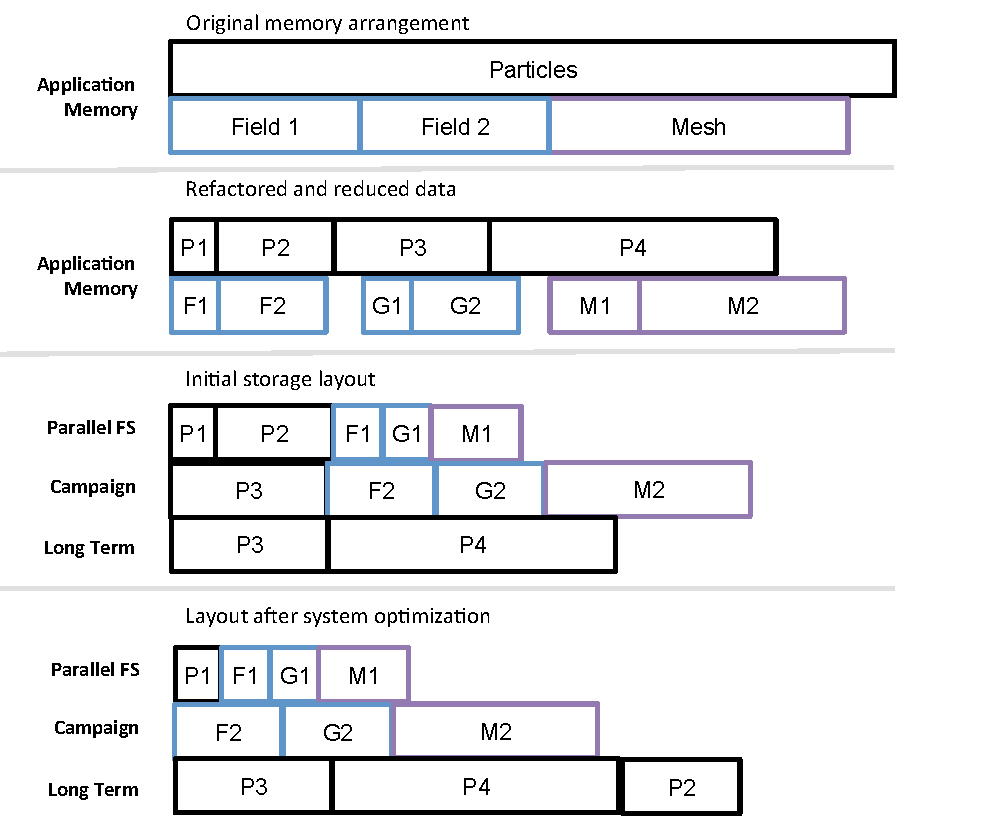
\includegraphics[scale=0.77]{graphics/SSIO-bucket.pdf}
        %\vspace{1ex}
        \caption{Data is given as a set of chunks which includes utility which contains the lifetime in a storage layer, and the priority of the layer.}
        \label{fig:ssio-bucket}
        \end{centering}
%        \vspace{1ex}
\end{wrapfigure}


We will design new techniques that users can use as part of a data mover, or
the system can automatically use, to raise or lower these sub-chunks up and
down the storage stack. The SSIO layer will then manage the system metadata so
that the user can transparently access any of these sub-chunks without
knowledge of the layer. This requires that when reading the data, the APIs will
then get a time estimate of reading, and then allow the users to determine if
they will read less (only the highest priority sub-chunks) if the time estimate
for reading exceeds their expectations. Existing Sirocco functionality may be
sufficient for these purposes, but it must still be proven in practice.
%

Users will also need to describe information about the data in order to choose
the ``most optimal'' data-refactoring routine. Currently, we understand that
users can tell us that the data represents: 1) phase-space (e.g., the particles
in our example), 2) spatial-changes (e.g., the mesh), 3) space-time (e.g.,
the fields on the mesh). We need this information to get the best possible data
refactoring methods. Although users can request a user-defined data-refactoring
method, system-level methods can use this information to make better decisions.
We will investigate new techniques and new semantics to take this information
and use this to best prioritize and re-organize information.

Finally we will investigate additional information on top of the data model.
This information will be used to indicate data associations that exceed
traditional data models. For example, the fields and mesh in our example have
an inherent relationship. A common data model will describe all of the
variables in the mesh (the coordinates, the units, and the types of elements if
this were a finite-element mesh). We will explore new mechanisms that will
group data together making it explicit that M1, F1, and G1 need to be organized
together.  In otherwords, in will not be helpful if data from M1 and M2 were
organized together along with only F1. When the users wants to visualize data
from the field, F1, they will need only M1 and M2 would be additional
information. Likewise, if the user wants to see F1 and F2, then they will need
the mesh from M1 and M2. This requires that the time to access all of this
data is approximately the same requiring similar access times for all of the
data.  We will investigate what choices the SSIO system must make in order to
keep these pieces ``together'', from a performance perspective. Can the storage
system move everything to a lower layer when all of it doesn't fit or is there
other, less tightly related data can be evicted to preserve the collective
retrieval performance?  We need to investigate the potential problems when this
occurs and how the users can specify additional information to ensure they get
the best possible data from the SSIO layer.

We seek to provide dynamic runtime information to the user and make the
system more transparent. The end user could analyze or visualize data in a more
predictable way since they have confidence how much longer they have to wait
for the data.

%Firstly, we will explore the augmentation of I/O application programing
%interfaces (I/O APIs) to allow applications to both specify timing and quality
%information and also query the storage system for timing estimates. If user
%decide to write or read data to or from hierarchical storage systems, they
%will rely on the API to send their intentions for inquiry and examine the
%system status, including how much data they would like to write/read, desired
%bandwidth, data compression method, etc, or the user can express their
%intension of writing data right now no matter what the traffic is now.
%Through this interface we expect the application and user to gain insights
%into how long a single output or input call will take given the required
%quality information, and then react to these estimates by adjusting the
%quality or restricting the scope of the data required. Likewise we will
%explore how an application can provide timing information to the storage
%system to allow the storage system to make optimization decisions to best meet
%the requirements from the application. 
%
%Secondly, we will also explore external data annotations, such as those
%provided by the configuration file in ADIOS. Through the use of these external
%augmentation the user can provide insights to the storage system on the
%relative value of the data, expected life time and performance
%characteristics, as well as relationships between different data sets. With
%this information the storage system can make optimizations specific to a use
%case. We expect these augmentations to be particularly important for eviction
%of data from a storage layer, and migration of data sets to a different
%storage layer. 

\paragraph{Challenges:}
These new techniques offer both technical and adoption challenges. We will only
consider the technical challenges. The proposed techniques and features aim to
expose broad system level environmental information to the application and
allow the application to adapt dynamically based on this information.  One
aspect of this challenge is the design of an interrogative API that offers a
negotiation between the application and the storage system to make adaptation
decisions.  Since we will work closely with many of the leading LCF
applications, we need to make sure that our additional APIs and semantics in
the storage layer will be accepted by these applications and eventually by the
rest of the community. This requires careful examination of all possible
design choices to ensure stable APIs and semantics that do not burden the users
with confusing APIS and semantics that cannot even be used by the system.


 % includes data-desc, apis, and qos-app.   

% \subsection{Application Interface}

%\subsubsection{Description of Data}

content



\subsection{Data Refactoring}



It is useful to classify scientific data into two basic categories: structured
data (in the sense that it satisfies a known or relatively simple model) or
unstructured data (in which information content follows no obvious or explicit
model).  Although scientific data generally contains random components (due to
finite precision, measurement and calibration effects etc.), scientific data is
never purely random. Broadly speaking, the path from data to knowledge consists
of extracting underlying models or patterns from the datasets, and interpreting
the resulting models. 

Ideally, the scientist would perform the analysis stage {\em in situ} to
extract the relevant information and, in the unlikely event of this being
possible, would effectively circumvent the large data issue completely.  The
problem of course is that this is unlikely to be possible since, by their
nature, large scale simulations aim to discover new information that is often
hidden as higher order effects amongst the data deluge. In particular, this
means if data thinning or truncation is applied then one is in danger of
effectively throwing out the baby with the bath water. One cannot store the
entire data set in easily accessible source, due to sheer size, yet one cannot
reduce it prior to archival without risking losing the information one is
trying to extract.  

Viewed in this way, the problem would appear intractable. However, the above
discussion fails to recognize that much of the data is redundant in the
information theoretic sense.  That is to say, the amount of information
contained in the data is often significantly less than the amount of data.  The
difficulty stems from the fact that one does not know about this redundancy in
advance. 


We propose a fresh approach to tackle the data overload problem head-on through
using preprocessors in which information is not simply stored in the form of
raw data, but rather in the form of appropriate parameterized algorithms. A
priori information on the nature of the data is used to choose the basic
algorithm while the actual values of the data are used to tune the parameters
used in the reconstruction procedures. We shall refer to this paradigm as an
Auditor.

Scientific data is sometimes described as essentially incompressible owing to
noise and other random effects present in the data, stemming from the numerical
algorithm, software implementation, system specific behavior etc. The reasoning
behind the description lies in the mathematical fact that it is impossible to
achieve lossless compression on completely random data sets \cite{Gray:book}. Even
recent state of the art lossless compression approaches \cite{GomezCappello} are only
able to obtain 15\% improvement in lossless compression ratio while reducing
the time spent in compression of floating point data by one half in some cases.
Nevertheless, these limitations apply only if one ignores two key features:
Firstly, randomness in scientific data generally occurs only below some
threshold related to the accuracy of the measurement apparatus or the numerical
algorithm. Secondly, lossy compression is perfectly acceptable provided the
loss level falls below this threshold.

Data compression broadly consists of three basic steps: (1) Pre-processing to
extract as much structure as feasible. This step is variously referred to as
filtering, preconditioning, and pre- processing but in all cases, the objective
is to represent the data in a form that becomes more amenable to compression.
(2) Removal of redundancy such as omission of duplicates etc.  Finally, (3) the
resulting data is compressed using entropy coding. The level of compression
that can be achieved in the final step is limited by the Shannon information
content of the data \cite{Gray:book}, and many standard tools are available for
efficient and perfect entropy coding. The potential for compression through
removal of redundancy is generally minor. The main scope for achieving
significant compression (a compression rate of two or better say) therefore
lies in the pre-processing step.

Research in the construction of pre-processing techniques is still in its
infancy, especially in context of exascale simulations. Techniques that have
been advocated range from simple difference filtering, bit-sorting, prefix
transformation through to simply reordering the data.  What these, and other
catchall methods, fail to exploit is a priori information on the nature and
provenance of the data.

As we have already observed, the incorporation of a priori information of this
type is vital if one is to obtain significant data reduction. The use of an
Auditor as a pre-processor exploits the wide (and increasing) cost gap between
CPU operations versus storage-based operations. The preprocessor would ideally
be employed in situ and is used in a similar fashion to pre-processors in
standard compression approaches such as FPC \cite{BurtscherFPC} in which an XOR
operation against the previous data is used as a pre-processor. The fact that
even such a crude pre- processor is able to deliver reasonable results augurs
well: Even a relatively crude Auditor can be expected to significantly
out-perform the XOR and other similar approaches.





 % includes data-reorg and the api specs move to the above section -
%\subsubsection{Data Reorganization Techniques}
One of the key element to get efficient data access during reading is the re-organization of the
data to ensure that the data that will be read back will involve minimal seeks on the file system 
along with aggregating similar data together to get optimal performance and placing the data
across multiple disks to get high levels of concurrency during reading. We will create APIs to
allow users to group similar data together in a data-model, and annotations (initially done in the
ADIOS layer) to allow relationships of variables to be expressed. We will then investigate both
system (general) data-re-organization techniques based on the utility of data and the relationships
of the data, and application-specific routines (for our initial set of evaluation test cases).  Once
we can generalize the application specific routines to a set of motifs, we can then allow this piece
of code to propagate to the general routines. In all cases we will investigate re-organizing the data
into an integer (most likely 8) bins, where they fall into the most likely accessed data to the least
likely accessed data. These methods will NOT be used for checkpoint restart data, since this
data needs to be accessed exactly how it is originally in memory.  We generally see that these
techniques are highly useful for analysis and  visualization data, where users can inherently place
their intentions of the data (life time of the data for eviction policies, prioritization of data 
importance). 


\paragraph{State of the art:}

\paragraph{Proposed research approach:}
General methods to re-organize the data fall into the following categories
\begin{itemize}
\item Precision based re-organization. This is where the most significant bytes of the data are
all group together from each object. This data generally will have a higher utility then the data with
the least significant bytes.  This process has the following three steps which need to be
efficiently implemented when data gets placed to the storage system and from the storage 
system. 
%
First, the data needs to be re-arranged which involves memory operations and needs
to be done in-situ. This operation involves no communication.  Data needs to be copied, so
the memory requirements are increased. At most this requires two copies an individual dataset
in memory, and we will investigate techniques to allocate and deallocate this memory if the user
will specify that the data will be overwritten after it is written to the storage system. This is often
the case for many of the data quantities written form the simulation, but there are many cases
where, for example, we want to write all of the particles from a Particle In Cell (PIC) simulation. 
Since the particles will be used later in the calculation, we need to duplicate the storage. Our
observation with working with the XGC1, GTC, Warp, and PiconGPU simulations (all leadership
class simulations) is that we can temporary increase the storage of the particles, and then 
release them since the temporary arrays used in the calculations are often freed when a PIC
iteration is finished.. 
%
The second step to give the metadata that allows the system to understand that an object is now contained in multiple bins of data. One of the challenges is the ability to bring together multiple bins
of data together (the high priority data along with the medium priority data) efficiently when the 
data is being read.  One research question is how we can manage the metadata efficiently.
We propose to place this knowledge into the middleware which will communicate this to the 
storage system.  This will give the storage system potential ways to increase the concurrency 
when accessing this information. For example, we can place the highest priority bits of an object
on the fastest storage system, and the next level of importance in the campaign storage. If a 
user request precision to a level where we need to access both, concurrently we can be
accessing this data, and moving the data to memory where it can be re-arranged. 
%
Since data will be placed in different bins along the hierarchy we will need to understand how
to initially place this in the fastest storage, and then evict this from the fastest storage without
effecting the performance of the simulation which is generating this data. Policies must be 
placed to ensure that we do not create any internal interference during these operations. We
will investigate doing this with ``meta-bots'' first introduced in the LWFS project and have 
these bots move the data.{\bf probably belongs in a different section} 

\item Frequency-based re-organization. FFT, Wavelets.
Another common technique to classify the importance of data is to first re-organize the data
in frequency space and then specify that as the frequency increases the importance of data
decreases. This allows us to place the lowest frequency pieces in the fastest storage, and
the highest frequency either on the slowest storage tiers, or if the data sizes are prohibitively  
costly, not even write out the highest frequency. This binning of data in frequency space can
take as an input (storage bandwidth knowledge, storage size limitations, and user intentions
of how long the majority of the data will be frequently accessed. 

These operations also require data transformations (for example an FFT and an inverse FFT)
and then re-arranging the data in real-space once we re-organize this. The research questions
we must address are: 1) what is the cost of re-organzing the data, 2) how do we 

\item Histogram binning. Re-organize the data through histograms to ensure we have enough
phase-space coverage. Where we have finner coverage we can move that data to other
quantiles of the storage. 

\item Multi-resolution. Traditionally we can look at every other point, and have a good feeling that 
this data will give a good estimate of the data.

\item Region of Interest. Using error techniques similar to AMR, we can understand where there
is data changing more rapidly and save this data at a higher resolution version than the smoother
regions of space.
{\bf Mark: can you fill these out much more and talk about the new techniques we will work on}.
\end{itemize}
\paragraph{Preliminary work and results:}
Text here
%%% Local Variables:
%%% mode: latex
%%% TeX-master: "../proposal"
%%% End:



%\subsubsection{QOS in the Application}
%proposed idea
A key insight in this proposed project has been the increased interaction of
the application with the storage system. Towards this end, we propose to
address the quality of service requirements by porivding the application
with mechanisms to specify the quality of I/O service, interrogate the
storage system, and react to the responses. Guided by our past work in
ADIOS\cite{lofstead2008flexible} we propose to explore the design of two
mechanisms for this purpose. Firstly, we will explore the augmentation of
I/O applictation programing interfaces (I/O APIs) to allow applications to
both specify timing and quality information and also query the storage
system for timing estimates. Through this interface we expect the
application and user to gain insights into how long a single output or input
call will take given the required quality information, and then react to
these estimates by adjusting the quality or restricting the scope of the
data required. Likewise we will explore how an application can provide
timing information to the storage system to allow the storage system to make
optimization decisions to best meet the requirements from the application. 
%
Secondly, we will also explore external data annotations, such as those
provided by the configuration file in ADIOS. Through the use of these
external augmentation the user can provide insights to the storage system on
the relative value of the data, expected life time and performance
characteristics, as well as relationships between different data sets. With
this information the storage system can make optimizations specific to a use
case. We expect these augmentations to be particularly important for
eviction of data from a storage layer, and migration of data sets to a
different storage layer. 

%execution
We will design an updated I/O API that will expand on the current POSIX I/O
semantics by adding new information to the I/O request. We will explore the
set of application level hints that can be easily provided to the storage
system in order for the storage system to make the most appropriate
optimization decisions. In particular, we expect the application to provide
hints on the length of time before the output data is persistent and
visible to users, and the expected lifetime of the data for data output
calls. For read calls we expect the set of hints to combine latency and
precision requirements. Additional hints will also be investigated. 

We will also develop a new type of querying system that allows application
to ask the storage system about completion timing information, the response
being an estimate provided by the storage system. We will explore how these
query functions can be integrated into common applications with minimal code
disruptions, and the set of policies that applications can use to respond to
this new information. We will also explore how applications can query the
storage system to gain insights on available space in different tiers and
how applications can tailor their output data to match the available space. 
Finally we will study the use of an external data annotation system that can
provide information to the storage system without requiring the application
to be recompiled. 

\paragraph{Challenges}
The design of new APIs posses both technical and adoption challenges. Here
we will only consider the technical challenges. The proposed set of APIs aim
to expose broad system level environmental information to the application,
and allow the application to adapt dynamically based on this information.
One aspect of this challenge is the design of an interrogative API that
enables a back-and-forth between the application and the storage system to
enable the application to recieve enough information to make adaptation
decisions. 

%%% Local Variables:
%%% mode: latex
%%% TeX-master: "../proposal"
%%% End:

\subsection{Data Placement and Movement}
\newcommand{\Sir}{Sirocco}

The application workflows targeted in this proposal generate very large
amounts of data, which needs to be processed and analyzed before
potential insights from the simulations can be realized. 
In-situ and in-transit data staging approaches can alleviate some of the
burden on storage, leveraging available compute and memory resources on high
end systems to process the data close to where it is generated. 
However, given current architectural trends, emerging systems will have a
vastly great gulf between the computing capability (the capability to
generate data) and the storage capability (the capability to store the
generated data). Moreoever, the complexity and heterogeniety of the
architecture will introduce new tiers in the storage system. Instead of
being a flat, roughly homogenous space in which data can be stored, the new
storage hierarchy will be multi-tiered and greatly heterogeneous. 

To take advantage of these architectural trends, we propose a triplet of
data placement strategies. First, we will utilize the faster layer of the
storage hierarhcies, such as DRAM, NVRAM and remote NVRAM, as the target for
the initial write from an application. To mitigate the space concerns, we
will use the techniques described in Section~\ref{sec:refactoring} to
identify and partition the segments of data with the highest utility for the
application and use case. The rest of the data will be stored on the
parallel file system, as is done today. Second, we will utilize the
migration of data supported by the existing implementation of \Sir to move the
data to an appropriate tier. We will explore how migration can be guided by
a combination of the utility function defined by the application and the
resources avialable to the storage system. Knowing the specific structural
and semantic information (including relationships between data segments)
about the data will enable migration to partition the data further to
optimize access to data for reader. 
Finally, we will explore policies that combine the knowledge of data, its
utility to users, the cost of maintaining data in long term storage and
other metrics to decide how to purge irrelevant data from the storage
system. 

Thus we propose to advance the state of the art in three connected areas:
(1) Data placement,
(2) Migration,
and (3) Purging. 

\subsubsection{Data Placement}
\label{sec:data-placement}

Our past work on data
staging\cite{tongipdps15,qiansc15}\cite{docan2012dataspaces}\cite{abbasi2010datastager}
in HPC systems, coupled with the experience in developing high performance
I/O transports for ADIOS \cite{liu2014hello,lofstead2008flexible} has
provided us with insights on how to manage the complex I/O requirements for
exascale applications, particularly in the face of the aforementioned
multi-tier storage hierarchy. A key requirements is application-driven
%
runtime mechanisms for dynamically managing data placement across the layers
of the distributed storage hierarchy,
%
coordinating data movement 
%
and data sharing between the components of the application workflow so as to
maximize its utility to the application and reduce access costs. Our
approach to data placement will leverage the increased set of knowledge
about the data available to the middleware and storage system, potentially
allowing for greater optimizations as compared to other storage solutions. 
The key components of our research include

\paragraph{Application Hints:}
As described in Section~\ref{sec:refactor} one of the main components of our
proposed storage system is the ability to refactor and reduce data as it is
generated, and to reorgnized and regenerate the data as it is accessed. We
carry this principle into the placement and movement of data by allowing
applications to define hints and policies that guide \textbf{what} data is
placed \textbf{where}. We will explore the use of application hints in two
distinct areas. Firstly, we will study the challenges and tradeoffs of either
augmenting the I/O interface with hints or allowing the additional of an
external specification that defines the use case. Our experience with
developing modern I/O interfaces has shown that both techniques have value,
and we will investigate the set of hints that are embedded in the
application code vs. those that are described within an non-compiled
specification. Secondly, we will study how hints can guide the initial data
placement as data is handed off from application to storage ( during a
write) and from storage to application (during the read). In both cases we
will study what minimal set of annotations and hints can allow the storage
system to minimize data movement and optimize the resources consumed by I/O. 

\paragraph{Data Utility:} We will formulate the concept of utility (from an
application perspective) that is assigned data objects to quantify the
benefits of placement and/or movement actions to application. These
utilities may be based on the importance of the data objects, the frequency
with which they are accessed, etc., and are used during runtime data
management. For example, data objects will higher utility value may be
placed closer (e.g., in faster memory) to the accessing application.
Similarly, when it is time to evict data objects from a higher level storage
layer, the decision about which object to evict may take the utility into
account.

\paragraph{Autonomic in-transit data management:} 
Efficiently placing data objects
vertically across multiple memory hierarchy layers and storage levels as
well as horizontally across different storage nodes requires balancing
competing objectives. In this project we will explore autonomic data
management strategies that can evaluate utility/cost tradeoffs and
appropriately place/move data objects at runtime. The autonomic approach
will leverage both user hints and information gathered at runtime (e.g.,
runtime data access history, network topology, etc.) to place data object.

\paragraph{ Runtime tracking and estimation:}
Autonomic data placement and/or
movement will leverage the information gathered at runtime together with
predictive analysis requirements. This information may include runtime
spatial-temporal data access patterns, physical network topology
information, and etc., which will be tracked and gathered at runtime, and
then be used to estimate and predict the behavior of coupled applications in
the rest of simulation-time. A key research aspect here will be to
anticipate accesses, for example using learning techniques or using
application knowledge, and use this information to prefetch data objects.
For example, we will identify and catalogue key phases and access patterns
in the target workflows and then use it to characterize patterns at runtime
and trigger appropriate place/movement actions.

\paragraph{State of the art:} NAND flash-based devices are being
increasingly used in HPC storage systems at different levels and for a
variety of purposes. Several studies such as \cite{multitier}, \cite{sc10li}
have investigated using compute node local SSDs as storage buffers, for
example, to temporarily cache checkpoint data to support recovery from
failures. Research efforts have also explored using deep memory devices for
data analysis. Active Flash \cite{activeflash} proposes in-situ scientific
data analysis by directly executing data analysis tasks on emerging storage
devices. Minerva \cite{minerva} extends the conventional SSD architecture
using a FPGA-based storage controller to offload data or I/O intensive
application code to the SSD to accelerate data analysis. However, these
solutions cannot deal with coupled application workflows, where the data
exchange and access patterns can be both complex and dynamic. Furthermore,
some of these solutions require hardware modifications or special access
priorities to the HPC systems, which can limit their use to specific
resources.

\subsubsection{Migration}
\label{sec:migration}

One important research question in this proposal is whether and how a liberated
Hierarchical Storage Manager designed for online use, such as Sirocco, might be
employed in supporting the higher level concepts discussed previously.
Conceptually, in this effort, data is accessed by the middleware IO libraries
at various tiers in the lower-level storage hierarchy. While Sirocco does
autonomously group the distributed set of media into like groups and manage
movement of data between these groups the various motivations to do so include
both the traditional ones found in classical HSM (Hierarchical Storage
Management) as well as the novel.

Sirocco groups like media into aggregated volumes on a service node, and like
service nodes with like media into pseudo-tiers. It accomplishes both using
attributes such as latency to first byte, bandwidth to and from the media, and
some function representing the resilience capabilities of the attached media.
In addition to these static attributes, when grouping servers into
pseudo-tiers, Sirocco also may employ more dynamic attributes such as CPU load
and the rate-of-change of the media use.

Grouping into pseudo-tiers is not a formal, nor rigid, concept within Sirocco,
at present. In classic HSM the tiering is often a formally expressed concept,
embodied both in the architecture and the implementation. In Sirocco, though,
it is not directly expressed. Instead, a client or server that attempts to make
a decision relative to migration and staging uses the attributes discussed
above to constrain the choice of candidates. For instance, a server acting as
an off-node writeback cache for a compute node might only have access to
volatile dynamic RAM for use as storage media and a client might deposit data
that is marked for persistent media as a resilience constraint. At some point,
then, such a server must copy or move the data to another Sirocco server with
media matching, or exceeding, the resilience constraint. At that point in time,
all servers managing appropriate persistent media are candidates but
second-order attributes, such as latency and bandwidth of a candidate's managed
media would tend to dominate the ranking. Thus, the concept of a ``tier''
becomes an artifact of decision rather than a formal concept.

Further complication arises when a Sirocco server is forced to make choices for
capacity reasons. The Sirocco architecture dictates that a server function as a
victim cache. As media managed by a server fills the server will begin to
manage for capacity. In order to do so, currently, it need only verify or make
a copy of the data on another server that meets the resiliency constraint of
the held data prior to removing the local copy and in the current
implementation the server makes no attempt either to remember it ever had the
data or to notify others about what it is doing.  others that it has removed
the local copy or remember that it has 

Taken together then, the above at least complicates the higher level research
questions discussed in this proposal, potentially even renders some
unachievable since a few involve determinism. We are forced, then, to consider
either or both mitigating management policies within and between Sirocco
servers as well as explicitly allowing clients to participate in capacity
management decisions, for a time at least, on the relevant Sirocco servers.

Our research intent involves short term and long term activities. In the short
term we will modify the relevant clients to provide hit and miss related data
and associated activities and explore an enhancement to our storage servers
that would provide some, hopefully tightly, bounded estimate about time to
first byte for a potential read operation. In the long term we hope that an
augmented client-server API providing usage hints will allow us to modify local
server policy algorithms to more effectively manage it's media and communicate
to other servers holding copies of the relevant data how they might best manage
theirs. In the event that this approach proves ineffective at meeting the
overall approach described in this proposal we will explore modifying Sirocco
servers to provide notifications about locations of the relevant data as they
migrate and stage as well as supporting client-directed pinning of location,
for a period at least. Client-directed pinning could introduce potentially
serious negative impacts to Sirocco's overarching goals though, since the
fundamental design of Sirocco assumes much about opaque and unrestricted data
movement, so this is contemplated only as a last resort.

\subsubsection{Purging}
\label{sec:purging}


% The title might have to change...

\paragraph{Background:} There is a spectrum of approaches on how
to leverage a memory and storage hierarchy: On one end of the
spectrum is to copy or move data from one tier to another, the
closer the tier to the hierarchy's top, the faster the access to
the data it contains. On the other end of the spectrum is to use
higher tiers exclusively for auxiliary data that to some extent
represents the actual data on the lowest tier. Examples of auxiliary
data are views, indices, lossy compressions, lower resolution data,
and summary data (sometimes also known as metadata). There are a
number of drivers that push approaches to one or the other extreme:
(1) if a high tier has sufficient room for an application's working
set, approaches that move the working set into that tier will perform
well; Conversely, if a high tier very rarely captures working sets,
it is better to fill it with auxiliary data that speeds up access
to the working set captured by a lower tier; working sets only
reduce capacity misses but the concept can be generalized to the
likelihood of having the right data in place, i.e. proactively
moving data to high tiers accessed in predictable patterns reduces
compulsory misses as well; (2) if the application generates parallel
read/write requests and strong consistency semantics are important,
approaches that use auxiliary data to speed up access to persistent
shared data might yield better performance than approaches that
require coherence overhead to keep all copies on higher tiers
consistent; (3) if the application's access patterns are mismatched
with low tier access characteristics, a combination of approaches
that use auxiliary data and move data between tiers in order to
convert access patterns into a better match will perform well.

% Any other drivers?

\paragraph{Approach:} This spectrum enables interesting strategies
to manage space pressure on high tiers: instead of just evicting
pieces of data (blocks, pages, objects, files), one can free space
by ``thinning'' data so that accesses within more limited views or
lower resolutions can still occur without misses while requests
outside of views or higher resolutions can leverage the information
stored in auxiliary data. Conversely, data on a high tier can be
``enriched'' (e.g. turned into a higher resolution) if there is
value in doing so.

\paragraph{Related Work:} Mention Stanford's Legion system.

\paragraph{Challenge:} The decision on when to thin and when to
enrich data on a particular level depends on \emph{access patterns}.
Approaches that leveragee access patterns in application at national
labs has shown to greatly improve performance and reduce the amount
of overhead required for data management~\cite{he:hpdc13}. The
challenge is for applications to communicate these access patterns
to the I/O stack layers that manages tiers outside of the address
space. In the proposed work we will develop an abstraction for
\emph{locality} that allow applications or runtime profilers to
describe locality properties of access patterns, and implement
services that leverage locality properties to dynamically determine
the value of thinning or enriching data at a particular tier.
Consider the example of a road navigation system: the locality
properties of each navigation client are based on physical constraints
of speed, direction, likely resolution of map, and the fact that
clients almost never go offroad.

\paragraph{Preliminary work and results:} Our recent work \cite{tongipdps15}
explored a two-tiered staging method that spans both DRAM and solid state
disks (SSD). It allows us to support both code coupling and data management
for data intensive simulation workflows in a loosely coupled manner. In
addition, our application-aware adaptive data placement has demonstrated the
effectiveness of using user provided access information as ``hints'', and
runtime data access pattern history to improve data access efficiency and
overall end-to-end execution. Besides, additional data placement
optimization \cite{qiansc15} that leverages physical network topology along
with data access patterns has also demonstrated lower data access costs and
good scalability. Our work have been deployed and proven with real
applications, e.g., coupled combustion simulations (DNS-LES) that are part
of the ExaCT Exascale Co-design Center and coupled Fusion simulations
(XGC0-XGCa) that are part of the EPSI SciDAC on current high-end systems
such Titan at ORNL.


%%% Local Variables:
%%% mode: latex
%%% TeX-master: "../proposal"
%%% End:

% \subsection{Migration}

One important research question in this proposal is whether and how a liberated
Hierarchical Storage Manager designed for online use, such as Sirocco, might be
employed in supporting the higher level concepts discussed previously.
Conceptually, in this effort, data is accessed by the middleware IO libraries
at various tiers in the lower-level storage hierarchy. While Sirocco does
autonomously group the distributed set of media into groups and manage
movement of data between these groups the various motivations to do so include
both the traditional ones found in classical HSM (Hierarchical Storage
Management) as well as the novel.

Sirocco groups like media into aggregated volumes on a service node, and like
service nodes with like media into pseudo-tiers. It accomplishes both using
attributes such as latency to first byte, bandwidth to and from the media, and
some function representing the resilience capabilities of the attached media.
In addition to these static attributes, when grouping servers into
pseudo-tiers, Sirocco may also employ more dynamic attributes such as CPU load
and the rate-of-change of the media use.

Grouping into pseudo-tiers is not a formal, nor rigid, concept within Sirocco,
at present. In classic HSM the tiering is often a formally expressed concept,
embodied both in the architecture and the implementation. In Sirocco
it is not directly expressed; instead, a client or server that attempts to make
a decision relative to migration and staging uses the attributes discussed
above to constrain the choice of candidates. For instance, a server acting as
an off-node writeback cache for a compute node might only have access to
volatile dynamic RAM for use as storage media and a client might deposit data
that is marked for persistent media as a resilience constraint. At some point,
then, such a server must copy or move the data to another Sirocco server with
media matching, or exceeding, the resilience constraint. At that point in time,
all servers managing appropriate persistent media are candidates but
second-order attributes, such as latency and bandwidth of a candidate's managed
media would tend to dominate the ranking. Thus, the concept of a ``tier''
becomes an artifact of decision rather than a formal concept.

Further complication arises when a Sirocco server is forced to make choices for
capacity reasons. The Sirocco architecture dictates that a server function as a
victim cache. As media managed by a server fills the server will begin to
manage for capacity. In order to do so, currently, it need only verify or make
a copy of the data on another server that meets the resiliency constraint of
the held data prior to removing the local copy and in the current
implementation the server makes no attempt either to remember it ever had the
data or to notify others about what it is doing.  others that it has removed
the local copy or remember that it has 

Taken together then, the above at least complicates the higher level research
questions discussed in this proposal, potentially even renders some
unachievable since a few involve determinism. We are forced, then, to consider
either or both mitigating management policies within and between Sirocco
servers as well as explicitly allowing clients to participate in capacity
management decisions, for a time at least, on the relevant Sirocco servers.

Our research intent involves short term and long term activities. In the short
term we will modify the relevant clients to provide hit and miss related data
and associated activities and explore an enhancement to our storage servers
that would provide some, hopefully tightly, bounded estimate about time to
first byte for a potential read operation. In the long term we hope that an
augmented client-server API providing usage hints will allow us to modify local
server policy algorithms to more effectively manage it's media and communicate
to other servers holding copies of the relevant data how they might best manage
theirs. In the event that this approach proves ineffective at meeting the
overall approach described in this proposal we will explore modifying Sirocco
servers to provide notifications about locations of the relevant data as they
migrate and stage as well as supporting client-directed pinning of location,
for a period at least. Client-directed pinning could introduce potentially
serious negative impacts to Sirocco's overarching goals though, since the
fundamental design of Sirocco assumes much about opaque and unrestricted data
movement, so this is contemplated only as a last resort.


% \subsubsection{Eviction Metrics}

% The title might have to change...

There is a spectrum of approaches on how to leverage a memory and storage hierarchy: On one end of the spectrum is to copy or move data from one tier to another, the closer the tier to the hierarchy's top, the faster the access to the data it contains. On the other end of the spectrum is to use higher tiers exclusively for auxiliary data that to some extent represents the actual data on the lowest tier. Examples of auxiliary data are views, indices, lossy compressions, lower resolution data, and summary data (sometimes also known as metadata). There are a number of drivers that push 

%\subsubsection{Policies}

Jay


%\subsubsection{APIs}

The new APIs will provide new functionality of specifying selectable performance/quality/- cost tradeoffs from both the application and system perspectives based upon the user guided rules/policy and runtime system monitoring status. It allows the middleware to make best possible decisions from the feedback of storage system knowledge, such that it will embed user intentions and the available system storage. The user would like the ability to get a certain amount of Quality of Service such that they can then make decisions when the expected bandwidth, for example is less than what they desire and will then place in a certain set of rules which the system can make autonomic decisions to help decide what should be done. We want the system to give the users a certain amount of currency in terms of bandwidth, storage space on each level, and latency expectations. These notions will be fuzzy but they will allow the user to make ad-hoc decisions to figure out what needs to be saved.

When user ask the system to write their data, and they would like to get an estimated time which they can then figure out, through a series of rules, whether they want to write out all of the data or wait for a later time to write or write a reduced amount of data. The decision is based upon if the system monitoring model could give us the estimate time during the reading and writing process, so that rules can be in place from the user perspective to make adaptive decisions. 

We will extend ADIOS with new APIs to provide such functionalities. If user decide to write or read data to or from hierarchical storage systems, they will rely on the API to send their intentions for inquiry and examine the system status, including how much data they would like to write/read, desired bandwidth, data compression method, etc, or the user can express their intension of writing data right now no matter what the traffic is now. After receiving the negotiation signal, the API return value will contain the estimate time of write/read data, potential bandwidth, concurrency, etc. User will adapt their decision from the system feedback and determine how much data they will write/read if the estimated time is too long for them. 

The capability of APIs provide dynamic runtime information to user and make the system more transparent to them rather than a black box. The end user could analyze or visualize data in a more comfortable position, where they are able to envision how much longer they are going to wait for data. 


% \subsection{Storage System}

%\subsubsection{Resource Management}

Jay


\subsection{Resource Management and QoS}
\label{sec:qos}

\subsubsection{Resource Management}
\paragraph{Background:} There is an important connection between finding the resources
that can fulfill a particular request and the performance predictability of that request. As such, this demands
careful resource management strategies that can deal with placement and retrieval of 
a large number of data chunks spread across the entire storage hierarchy. 
%This connection is particularly important for data retrieval 
%- in large scale storage systems, finding a resource to read can be a significant, if not dominant, 
%component of overall read latency. 
Locating resources is a typical distributed systems problem. Centralized solutions are limited in their
scalability, because they require a single entity that tracks updates in the system. 
Traditional file systems are good examples for this - most updates to files require updates 
to their centrally maintained block allocation tables. 
The opposite of file systems are ``pile'' systems, which, instead of keeping track of updates, searchs for 
resources at request time. Pile systems allow very efficient writes because clients can write wherever
there is free space and there is very low bookkeeping overhead. However, unbounded search in pile systems
is possible, e.g., when it is unclear whether the resource actually exists. 
Methods to make searches more efficient without reverting to centralized bookkeeping usually involves 
partitioning of the search space and a method to limit the search to a small number of partitions. 

Frequently this involves a hash function that is relatively stable against changes to its range, 
such as failures or updates to the hardware of the system. Consistent hashing~\cite{karger:stoc97}
is scalable since it can be well-known throughout a system of any size and only requires minimal 
movement of data in the presence of failures or system changes. 
%Consistent hash functions can also
%have sets of ordered but infinite lists as their range (which works well with primary replication)
%~\cite{honicky:ipdps04}, implement declustering (limiting overlap between partitions), and support
%placement policy rules~\cite{weil:sc06}.

\paragraph{Approach:} 
In this proposal we will investigate the trade-off in terms of predictable performance between 
``filing'' data, making an upfront investment to ensure finding data quickly, and ``piling'' 
data, pushing the cost of finding to the moment when the data is actually needed. {\color{red}This trade-off 
has a parallel in data management where there are two alternative paths to achieve knowledge: 
the analogue to filing is ``extract, transform, and load'' (ETL) data into a warehouse, paying 
an upfront ingest cost to achieve fast querying; the analogue to piling is to not pay any upfront 
cost and query the raw data directly by using data processing platforms such as Hadoop sentence CHECK-tsr}. Recent work 
has found that the combination of these two techniques can be optimized to perform better than 
any one technique alone~\cite{lefevre:sigmod14a}. We believe that a similar opportunity exists 
for combining filing and piling approaches to achieve performance predictability without sacrificing 
too much flexibility.

More specifically, the coarseness of a search space partitioning limits the search time within 
a partition, i.e. finely partitioned search spaces require little or no search within a partition 
but offer little placement flexibility. Partitioning can also be fine in one dimension, and coarse 
in another to allow flexibility where it is most needed while still ensuring fast finding. For 
example, a hash function can finely partition a low storage tier but each partition can extend 
across multiple tiers so that a search still has to occur in order to find a resource on a particular 
tier.  

%Specifically, we will address the following research questions:
%\begin{tightItemize}
%  \item Can we make any guarantees in a scalable decentralized system?; 
% \item  What quality of service metrics can be make guarantees on in a scalable
%    way?;
%  \item What kind of error rates will we have in our estimation and what error
%    rates are acceptable?;
%  \item How much will the qos scheduler, admission control, manager cost in
%    terms of resources and time?;
%  \item  How do we make the scheduler scalable with the size of the system?
%\end{tightItemize}

\subsubsection{QoS}
\paragraph{Background:} QoS refers to the
properties of the performance quality of a particular service, in
this case the storage system.
%Performance quality can be expressed in either relative or absolute
%terms. Examples of relative performance terms are ``fair'',
%``proportional'', or ``priority/class-based'' (``the higher the
%priority the better the service'' or ``1st class is better than
%2nd''). The key advantage of relative performance terms is that
%they are easy to implement. The key disadvantage is the difficulty
%of making any guarantees based on those implementations --
%even relative guarantees are mired by the well-known effect of
%priority inversion~\cite{lampson:cacm80}. Examples of absolute
%performance terms are ``rate-based'', ``soft real-time'', and
%``hard real-time''. The key advantage of absolute performance
%terms are that they enable the implementation of strong
%guarantees: absolute terms enable agreements between application
%tasks and storage that we call \emph{reservations} and that do not
%change meaning depending
%on the storage system's workload. The key challenge of absolute
%performance terms is that their implementation is non-trivial,
%especially in large-scale systems.
One of the key differentiating features this project offers is driving storage
decisions through QoS \emph{reservations}, rather than continuing the current model
of allowing applications to compete freely without restriction, for part or all of the storage
resources. This traditional approach leads to interference effects
\cite{lofstead:2010:io-variability,liu_hotstorage} that can greatly impact I/O performance predictability. 
%Further, with the introduction of additional tiers in the
%storage stack, the performance variability will increase with greater
%competiion for limited high performance resources. 
%% Temporaily commented out the above sentence, because it may not be true for the next DOE systems. 
Unfettered, this competition can yield a lower system and application performance 
than the case where applications attempt to reserve storage resources, thereby enabling the storage system
to reason over its performance in terms of reservations and actual
performance.
In the cases where an application arrives that needs to run more urgently
than any of the other already running applications, the system
can rapidly respond to it by reducing the amount of resources taken 
by less urgent applications, allowing the urgent application to finish,
and later reverting back to the previous committed resource level for the rest.
This can be automatically enforced via user- (or administrator-) specified \textit{policies}\S\ref{sec:data-description}.

There are two fundamental causes that can impede the I/O performance
in an extreme-scale SSIO system. One is indirection, where layers
of storage tiers are employed either for performance and/or for
scalability reasons.  The direct consequence is that there could
be multiple traversing paths from application end to the rest place
of data, and more often than not, the I/O paths are not under control
under any single authority. The other cause is the shared use of
resources. The best effort I/O request/response nature and lack of
QoS mechanisms imply that there is little guarantee in terms of
expected performance. Both indirection and shared use of resource
contribute to a high probability of imbalanced use of resources
thus the occurrence of congestion and degraded performance.

As an example to demonstrate that this disconnection will hurt
system performance: We launch 4096 processes with each process doing
a single file I/O operation against half of the Spider II file
system. The traces of those files are analyzed to examine the
utilization distribution of different components. Figure (a), (b)
and (c) shows the resource usage distribution for OSTs, OSSes, and
LNETs, respectively. We observe that there exists a significant
variation in usage across components of any given type (e.g., OST,
OSS or LNET). For example, some OSTs are used more than 10 times
while some others are never used (corresponding to zero frequency
count). Similarly, OSSes and LNETs show significant imbalance in
usage under the default placement strategy. Consequently, imbalanced
resource utilization increases the contention at certain components
more than others.

% Don't know how to integrate this. Gary
%Given these insights, we advocate the idea that the infrastructure
%knowledge should find a way to relay to the upper layer for better
%and more effective use of resources. We think this is more pertinent
%and critical given the recent development of multi-tier storage and
%storage component heterogeneity.  There needs to be a way for
%application/middleware layer to gain more exposure of storage system
%for more intelligent processing logic.  One prime example of such
%exposed knowledge can be request/response time. To most applications,
%this is a black box. Profiling it at the upper layer is neither
%efficient nor effective, as it doesn't reflect cross-layer
%characteristics. However, Most of storage layer does keep a detailed
%profiling of such information. We therefore envision and propose a
%histogram-based request/response profiling API that application and
%middleware layer can leverage and make more informative decisions.


\begin{figure}[tbh]
  \centering
  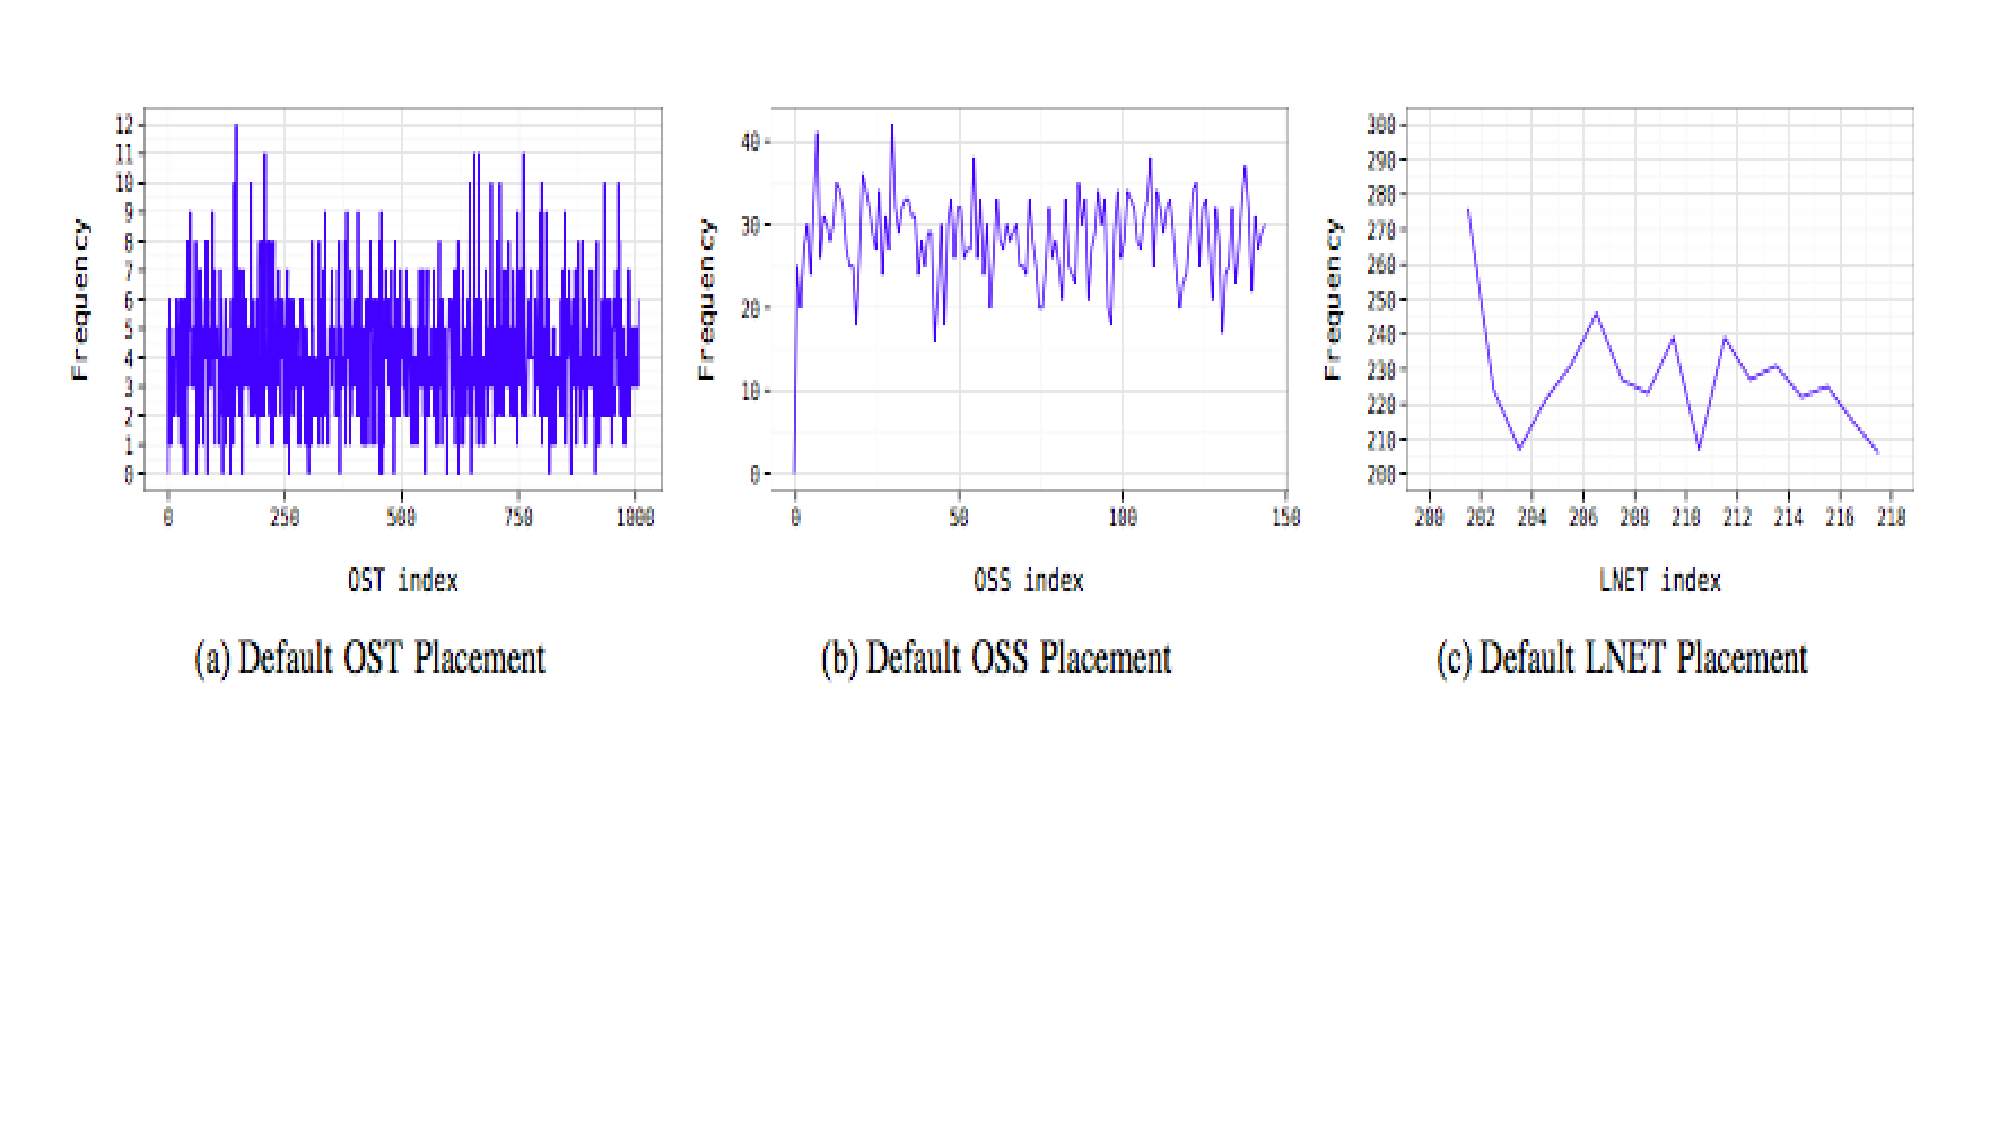
\includegraphics[width=\columnwidth]{graphics/infrastructure.pdf}\vspace{-1.2in}
  \caption{Resource usage distribution for OST(a), OSS(b) and LNETs(c) }
\end{figure}


% This is about finding the relationshiop of workload-dependent to workload-independent metrics. -- Carlos
 %are driven from multiple different approaches. First, supporting
%capability runs is a priority for capability machines. We propose to address
%capability run performance by incorporating monitoring for prepartory runs at
%smaller scale to profile the application output characteristics both from a
%writing velocity and volume, but also for example read patterns for the data
%analytics required to generate scientific insights from the raw data. 

% Not sure how to reuse this ... -- Carlos
%By
%discovering approximate data proportions that will likely be the key subsets
%targeted by the simulation run, we can generate a policy to preserve a certain
%storage portion for high fidelity data storagae and use slower or perhaps lower
%fidelity or compressed data storage for less interesting data portions. We will
%support spreading data appropriately across the storage hierarchy. In
%particular, we will investigate how to place data across different layers to
%meet the performance requirements for output while maintaining system
%availability for other applications and offering the best possible performance
%for the data analytics that will ultimately process this data.


% Not sure how to reuse this... -- Carlos
%Second, once data has been placed for future performance requirements, policies
%must be able to address maintaining data on a priority basis in that location
%to deliver on the placement optimization generated by the capability run
%profilier.

% This is a matter of metering, not performance reservations. -- Carlos
%Third, most future NVM devices have limited write endurance prompting
%management to ensure fair use by all machine users. Technologies like
%NAND-flash and Phase Change Memory have limited write endurance. By
%incorporating policies about the proportion of write endurance a compute
%allocation is entitled to, data placement decisions can be made to ensure fair
%resource usage. While the offending application will suffer worse IO
%performance, other applications that more carefully address their data
%intensity on these limited devices will achieve higher overall performnce. Only
%by instituting such policies can we encourage application users to adopt
%technology to manage the limited resources.


%We propose to investigate both offering a policy mechanism and how to implement
%these kinds of policies in a way that addresses offering the shortest
%end-to-end time for scientific insights.

% Lifted the following paragraph to the beginning. Gary
%``Quality of Service'' (QoS) refers to the
%properties of the performance qualtiy of a particular service, in
%this case the storage system.
%Performance quality can be expressed in either relative or absolute
%terms. Examples of relative performance terms are ``fair'',
%``proportional'', or ``priority/class-based'' (``the higher the
%priority the better the service'' or ``1st class is better than
%2nd''). The key advantage of relative performance terms is that
%they are easy to implement. The key disadvantage is the difficulty
%of making any guarantees based on those implementations --
%even relative guarantees are mired by the well-known effect of
%priority inversion~\cite{lampson:cacm80}. Examples of absolute
%performance terms are ``rate-based'', ``soft real-time'', and
%``hard real-time''. The key advantage of absolute performance
%terms are that they enable the implementation of strong
%guarantees: absolute terms enable agreements between application
%tasks and storage that we call \emph{reservations} and that do not
%change meaning depending
%on the storage system's workload. The key challenge of absolute
%performance terms is that their implementation is non-trivial,
%especially in large-scale systems.

\paragraph{Approach:} The goals of this proposal require applications
to demand guarantees in terms of absolute performance qualities.
The first key enabler for any service to make absolute guarantees
is \emph{performance isolation}, i.e. the ability to shield the
performance impact of one task from another. The most straight-forward
but least flexible strategy is to simply cap the latency of each
task, regardless of its completeness (see for
example~\cite{decandia:sosp07}). This strategy is applicable when
incomplete tasks still have value and missing results are either
not important or can be easily retrieved in subsequent tasks. A
more generally applicable strategy is to control the admission of
tasks to the system: \emph{admission control} maintains a
\emph{utilization model} that can predict the utilization of system
resources given a new task, estimates the current utilization of
the system, and decides whether the task can be admitted without
overloading the system. Thus, admission control avoids system
overload conditions that lead to hard-to-model chaotic behaviors.
Consequently, utilization models can frequently be approximated by
automatically calibrated linear models (see for
example~\cite{skourtis:hpdc12}).

Another essential component of performance isolation is the
\emph{charging model} which determines which task(s) should be
charged how much for a request. Performance isolation is implemented
by the charging model by ensuring that performance of a task only
depends on its reservation and its workload behavior (but not on
other workloads in the system). Each task has a budget based on its
reservation and spends it based on the cost of each request determined
by the charging model. A charging model determines the cost based
on the utilization model and the interactions a request can have
with other requests (e.g. a random request to spinning media
interrupting a stream of sequential requests).

Performance isolation (including its utilization and charging models)
critically depends on \emph{workload-independent metrics}. Even
though throughput and latency are frequently the most meaningful
metrics for an application, they are not workload-independent and
therefore are inadequate for measuring the utilization of a device
across all workloads, unless one accepts worst-case estimates that
can lead to gross underutilization of resources (e.g. the throughput
of random and sequential workloads in spinning media differ by
orders of magnitudes). A common workload-independent metric is
\emph{time utilization}, i.e. the amount of time a resource is
utilized in a given time interval. Time utilization has the advantage
of having an always defined maximum and therefore makes resources
fully reservable. Even though a workload-independent metric might
at first not appear meaningful for an application, given a particular
workload an application can discover the relationship between its
workload-dependent metric and the workload-independent metric.
Because of performance isolation, the application has to discover
this relationship only once.
To achieve effective performance isolation, we seek to expand the resource management
capabilities in Sirocco to support additional utilization 
metrics to guide resource management
decisions. Currently, Sirocco offers automatic resource management capabilities,
based on resource capacity and data resilience requirements, and it needs to be extended
to offer data-centric metrics that help guide the forced QoS decisions.

As stated in the introduction, we seek to make a storage stack that works with
the user. Towards that end, we must incorporate data attributes into this
process. For example, particularly for a capability run, the storage system
should give priority to data subset tagged with high importance to stay in fast
storage tiers. Enabling this priority will be driven by other job
characteristics such as job size or a manually set priority inserted by system
administrators. It should also store the highest quality data possible given
the performance requirement. Ideally, the storage system will store the raw
data at full fidelity. When this tier approaches capacity, data should migrate
not just based on age, but also based on this priority. This will help ensure
the shortest time to insight by making sure the most important machine runs
have priority to use system resources.

\paragraph{Related Work:} On current production HPC systems, absolute I/O performance
guarantees are not possible. Previous work \cite{lofstead:2010:io-variability,liu_hotstorage} 
from this project team uses a client-assisted approach to mitigate I/O variablity at scale (100,000-core).
Recently server side QoS scheduling has also been studied for HPC applications \cite{Dai:2014}.
However, the key hurdle of scalability has not been solved.
Existing efforts on scheduing resources~\cite{thapaliya:2014:io-cop,dorier:2014:calciom} attempt to offer
admission control to maximize storage performance. Unfortunately, these efforts
are limited to participating applications and only applications from a single
platform. For this approach to be effective, the storage system must offer an
approach that handles clients from all connected platforms and does not
require modification to use new storage access APIs. By using a priority
tagging system, we will offer defaults suitable for all applications that can
be informed by simple extensions to the job scheduler or more advanced
management through new APIs. On the other hand, storage QoS has been
studied for enterprise applications and systems \cite {Gulati:2007,Gulati:2010,Gulati:2012}
in virtualized environments. It is not straightforward to adapt these solutions
to HPC storage systems because of the scalability and efficiency concerns, despite
they achieved very good performance isolations.

\paragraph{Challenges:} The deep and heterogeneous memory and storage
hierarchy we are assuming for this proposal complicates the
relationship between workload-dependent and workload-independent
metrics: the performance of a task can significantly differ depending
on what levels of the hierarchy are involved. Furthermore, an
important goal of the proposed project is to enable applications
to reason about the trade-off between resolution and latency, adding
yet another dimension to how tasks are mapped to resources.

\begin{tightItemize}

\item A key challenge of admission control is scalability: the
decision of whether to admit a task could potentially depend on
global knowledge of the current utilization of every single resource
in the system. Scalability therefore depends on whether admission
control is able to accurately map a new task to a relatively small
set of resources which can quickly provide up-to-date utilization.
One approach might involve pseudo-random mapping that also load-balances
as a side-effect.

\item To offer latency/latency trade-offs, the system must be able
to quickly generate a number of data production plans, involving
different parts of the hierarchy and different data resolutions.
It will then use the utilization model to estimate the latency for
each production plan and the resolutions they can provide. Here
again, pseudo-random selection could reduce the number of resources
that would be involved, thereby increasing scalability.

\item The complexity of a utilization model involving the entire
storage hierarchy with 100,000s of devices is potentially daunting.
However, the utilization model can be simplified by modeling classes
of devices as well as classes of requests. In particular, each
device could restrict access to its content via a set of well-defined
methods with known, absolute performance properties.

\item Flash devices become inherently unpredictable when reads and
writes are mixed on the same device because of garbage collection.
While write latency can be easily hidden using asynchronous I/O,
hiding read latency is more difficult. By separating reads and
writes for each device, read latency becomes predictable. The
challenge is to minimize duplication of data, at least on fast
layers and leverage redundancy across layers.

\end{tightItemize}


%%% Local Variables:
%%% mode: latex
%%% TeX-master: "../proposal"
%%% End:


%\subsubsection{Discovery}

%
% This has been merged into the Naming Servie subsubsection
%

Hierarchical Storage Management (HSM) systems offer a strct caching approach
for managing different storage capacities trading off performance for capacity.
By maintaining a single namespace across all tiers, it is possible to list a
single directory view with files stored at different tiers. While this approach
to managing multi-tier storage works, it is far from ideal for scientific
simulations.

Our goal with this proposal is to offer a similar capability, but use a finer
granularity. Instead of a single file such as might be used to store an entire
timestep output for a simulation, we will demonstrate offering the same
capability at a subset of a single variable level. By shifting to a
finer-grained approach, we will enable more effective use of close/fast/small
storage tiers. Traiditional HSM stores an entire file on a tier making room if
insufficient space is available. With this shift to a partial variable
granularity, a 1 PB output with 500 GB of ``high interest'' data can limit this
costly tier ussage to just 500 GB greatly enhancing usability.

Tagging a variable subset as ``high interest'' requires intervention from the
application and/or middleware to determine what data meets this criteria. The
storage system itself simply needs to offer an ability to perform different
actions based on this information.

The challenge for discovery is that potentially, data will migrate from where
it is initially stored to a new location within the storage system. Sirocco
offers an ability to search for data that has moved as well as forcing a
particular resilience-based replica be the ``authoritative'' version. We will
investigate if the current Sirocco functionality is capable of supporting the
new operating modes we wish to offer. Initial expectations suggest having
bounded time guarantees for finding data are critical for offering the quality
of service guarantees we wish to offer. This new work will be an expansion of
Sirocco's currently planned features.

The other aspect of discovery is the negotiation between the user and the
storage system for a data quality/retrevial time trade-off. The naming service
will work hand-in-hand with the discovery, data migration, and time estimation
services to offer the best possible options for data retrevial based on quality
of service requested.


\subsection{Naming and Discovery Service}
\label{sec:naming-discovery}
\paragraph{Background:}
Given the well documented difficulties with POSIX-compliant naming and our
approach that decomposes what would be a single file into potentially large
number of objects, we must take a new approach to naming.  Data migration, as a
result of system pressures or user/system policies, further adds to the
complexity of managing naming and discovery. Our naming service must maintain
sufficient metadata information, track or be able to find objects as they move
across storage layers, and facilitates data discovery. Since we need to also
support access through POSIX APIs for existing application and system
integration, we must address how to bridge the drastic differences between the
decomposed objects of potentially varying fidelity with potentially multiple
versions with a POSIX API-compatible interface.

Hierarchical Storage Management (HSM) systems~\cite{blaze:1992:hsm} offer a
strict caching approach for managing different storage capacities trading off
performance for capacity.  By maintaining a single namespace across all tiers,
it is possible to list a single directory view with files stored at different
tiers. While this approach to managing multi-tier storage works for whole files
that fit on single logical devices, it is far from ideal for scientific
simulations.

The overriding theme for this proposal of providing a cooperative relationship
between the user and the storage system extends into this area as well.
Negotiating the data quality/retrieval time trade-off requires additional
metadata.  Providing this functionality requires the naming service be able to
both return a list of data versions and an indication of data quality. This
will be combined with a retrieval time estimate for each version by the
middleware to determine what data version should be retrieved.  This estimate
will be discussed elsewhere in this proposal.

In addition to the basic naming and data tracking operations, we will also need
to incorporate authorization capabilities. Sirocco currently integrates with a
Kerberos service for authentication. Given a capability ticket, a user can
access different objects as needed. This ticket structure offers protection
services typically offered on POSIX directories and files, but can do it at the
fork level instead. This allows a reduced quality data version to be available
for the general users while the high-quality version would be limited to the
data creator. This and other considerations for security must be incorporated
into the entire naming and metadata service.

While strongly encouraging data to stay in a particular type of storage tier,
ultimately it must be possible to flush this data to make room for other uses.
Sirocco offers a ``flush'' operation that forcibly migrates data to the
long-term resilience requirements, freeing space in the scarce resources. In
many, if not most cases, this will move data towards or actually on to a device
like tape, intended for long-term storage.

\paragraph{Approach:}
Our goal with this proposal is to offer a similar capability but with a finer
granularity leveraging the inner structure of scientific data. It must also
handle data discovery efficiently for cases where data is spread across several
storage layers or some of those pieces may have migrated based on system
pressures or user or system policies. Instead of a single file, such as might
be used to store an entire timestep output for a simulation, we will
demonstrate a metadata service with naming at the science variable level, but
with an associated list of all of the variable pieces and potentially different
versions stored throughout the storage system. By shifting to a finer-grained
approach, we will enable more effective use of close/fast/small storage tiers
and prioritize objects with high importance.  Traditional HSM stores an entire
file on a tier making room if insufficient space is available.  With this shift
to a partial variable granularity, a 1 PB output with 500 GB of ``high
interest'' data can limit this costly tier usage to just 500 GB, greatly
improving storage availability in the close/fast/small tier and focus
performance/capacity costs to get the most science from the platform.  By
only placing ``high interest'' data in the close/fast/small tier, we will
effectively reduce pressure forcing data migration hurting both writing
performance and the later data analytics required for generating scientific
insights.  Sirocco identifies a data segment using a
container/object/fork/address tuple that can have associated attributes. We will
add both a special attribute indicating that this record is of ``high
interest'' as well adapting a migration mechanisms to use this attribute, if
present, to strongly encourage keeping the record in  the highest storage tier as possible. 

Meanwhile, we need to be able to locate or ``discover'' the data should it
move.  The challenge for discovery is that potentially, data will migrate from
where it is initially stored to a new location within the storage system.
Sirocco offers an ability to search for data that has moved as well as forcing
a particular resilience-based replica be the ``authoritative'' version
migrating the data to a particular location. We will investigate if the current
Sirocco functionality is capable of supporting the new operating modes we wish
to offer. Initial expectations suggest having bounded time guarantees for
finding data are critical for offering the quality of service guarantees we
wish to offer. Some potential approaches can build on CRUSH~\cite{weil:ceph}
from Ceph to offer a map of where to search for data sequentially. Given our
multiple storage tiers, we would extend this using some mechanism to shift to
the next tier to continue searching because the requested data never made it to
this location. This new work will be an expansion of Sirocco's currently
planned features.

We plan to address scalability problems by continuing with the LWFS and Sirocco
model. LWFS and Sirocco have taken an approach similar to the pure object
stores, but with a focus on the HPC setting. They have abandoned a fully POSIX
compliant metadata service as the default model in favor of a
container/object/fork/address tuple for identifying data similar to those used
for pure object stores. By having a service that addresses the object
collections that comprise a single thing, such as a variable or timestep
output, just enough metadata is maintained to make the storage system usable
without additional heavy lifting by clients.  LWFS demonstrated a POSIX-style
namespace on the side kept in sync using a transaction process like
D2T~\cite{lofstead:2012:txn} showing that this alternative approach can support
traditional POSIX API calls even though the underlying storage system uses a
different model. Because we are not requiring the entire storage space be
addressible from a single tree root, we can offer multiple independent roots
using the Sirocco object storage. We will investigate how to make the naming
and discovery service scalable under the circumstances outlined above.

\paragraph{Related Work:}
Structurally, the traditional POSIX naming service offering a hierarchical
space consisting of directories and files may be maintained for backwards
compatibility. However, this view will not offer the same strict semantics
POSIX defines. We must break these strict semantics to address scalability
problems forced by the serialized access to a single source for creating and
accessing files.  Several efforts~\cite{patil:2007:giga+,carns:pvfs} have
worked to reduce this contention by doing things like reducing the serialized
scope to a single directory or subtree, or allowing a single process in a
collective file operation talk with the metadata service and distribute a
handle to other participants. While these approaches help, they do not address
this key scalability limitation of serialized access--even if the metadata
service is spread across multiple nodes. Instead, we will offer a short
duration to consistency POSIX view to offer the performance and consistency
requirements an exascale application demands.

While pure object stores, such as those popular in the big data
domain~\cite{Fitzpatrick:2004:memcached}, others avoid this bottleneck by
strictly offering an object ID with the application required to manage how this
ID maps to something of interest. This approach of removing the metadata
service from the system level completely can work well for scale out
applications where data is created or consumed by a single process at a time or
just in a work queue rather than potentially O(1 million) processes all
actively collectively for a single ``object''. To address this case, having
some system integrated metadata services to associate names with these object
is a preferable solution. While it will not have the same synchronous
consistency semantics as POSIX, we will offer something as close as possible to
address legacy application and command-line style data access and migration to
other storage types using these POSIX semantics.

\paragraph{Challenge:}
The main challenge of incorporating the additional, rich metadata will be
joined by the additional challenge of coordinating with the other storage and
application-layer services to offer the best access times possible for data
stored in the system. The developed metadata services that drive data
compression and subsetting operations must have easy, consistent, and ideally
non-blocking or locking access to this metadata service. We must investigate
how to build such a metadata and naming service that also incorporates and
maintains the additional metadata required to support our advanced
functionality.

Our research in this area will address the following questions:
(1) Since our metadata is distributed and partitioned, how do we respond to user
  requests within a specified time bound with accuracy? How do we estimate the
  completeness of the response?, 
(2) For POSIX API requests, how do we respond if only varying data fidelity
  levels are available for the requested data object?, 
(3) What level of metadata should we maintain and keep in sync to enhance
  response quality within time-bound requests?, 
(4) How much time should be allowed for searching for metadata given the user
  specified limits for data retrieval since the user will still have to spend
  the data retrieval time from different devices? How do we integrate the read
  time overhead into the metadata requests?, and
(5) How do we provide appropriate security while maintaining scalability,
  particularly with the distributed metadata stores?

\begin{tightEnumerate}

\item {\bf Milestone 1}: Demonstrate a metadata service capable of serving both POSIX
clients and our clients, but without consideration for authentication,
authorization, or data migration.

\item {\bf Milestone 2}: Demonstrate a time bounded search approach for finding data
within the storage system to identify data and the current location.  This will
update the cached information in the metadata service to short-circuit future
requests for the data presuming that it does not migrate again soon.

\item {\bf Milestone 3:} Demonstrate incorporating {\color{red}A\&A (what does this stand for CHECK-tsr)} and show scalability under
both application load as well as storage system pressures, showing that we can
tolerate both loads and maintain quality of service.

\end{tightEnumerate}


% \subsubsection{Estimation of Times}

Feiyi

There are two fundamental causes that can impede the I/O performance in an extreme-scale SSIO system. One is indirection, where layers of storage tiers are employed either for performance and/or for scalability reasons.  The direct consequence is that there could be multiple traversing paths from application end to the rest place of data, and more often than not, the I/O paths are not under control under any single authority. The other cause is the shared use of resources. The best effort I/O request/response nature and lack of QoS mechanisms imply that there is little guarantee in terms of expected performance.  Both indirection and shared use of resource contribute to a high probability of imbalanced use of resources thus the occurrence of congestion and degraded performance. Traditionally, there is a disconnection between storage infrastructure and rest of system software and applications: the infrastructure details are not exposed anywhere at all. One argument favoring this is to ensure a platform agnostic design. 

As an example to demonstrate that this disconnection will hurt system performance: We launch 4096 processes with each process doing a single file I/O operation against half of the Spider II file system. The traces of those files are analyzed to examine the utilization distribution of different components. Figure (a), (b) and (c) shows the resource usage distribution for OSTs, OSSes, and LNETs, respectively. We observe that there exists a significant variation in usage across components of any given type (e.g., OST, OSS or LNET). For example, some OSTs are used more than 10 times while some others are never used (corresponding to zero frequency count). Similarly, OSSes and LNETs show significant imbalance in usage under the default placement strategy. Consequently, imbalanced resource utilization increases the contention at certain components more than others. 

Given these insights, we advocate the idea that the infrastructure knowledge should find a way to relay to the upper layer for better and more effective use of resources.   We think this is more pertinent and critical given the recent development of multi-tier storage and storage component heterogeneity.  There needs to be a way for application/middleware layer to gain more exposure of storage system for more intelligent processing logic.  One prime example of such exposed knowledge can be request/response time. To most applications, this is a black box. Profiling it at the upper layer is neither efficient nor effective, as it doesn't reflect cross-layer characteristics. However, Most of storage layer does keep a detailed profiling of such information. We therefore envision and propose a histogram-based request/response profiling API that application and middleware layer can leverage and make more informative decisions.

\begin{figure}[tbh]
  \centering
  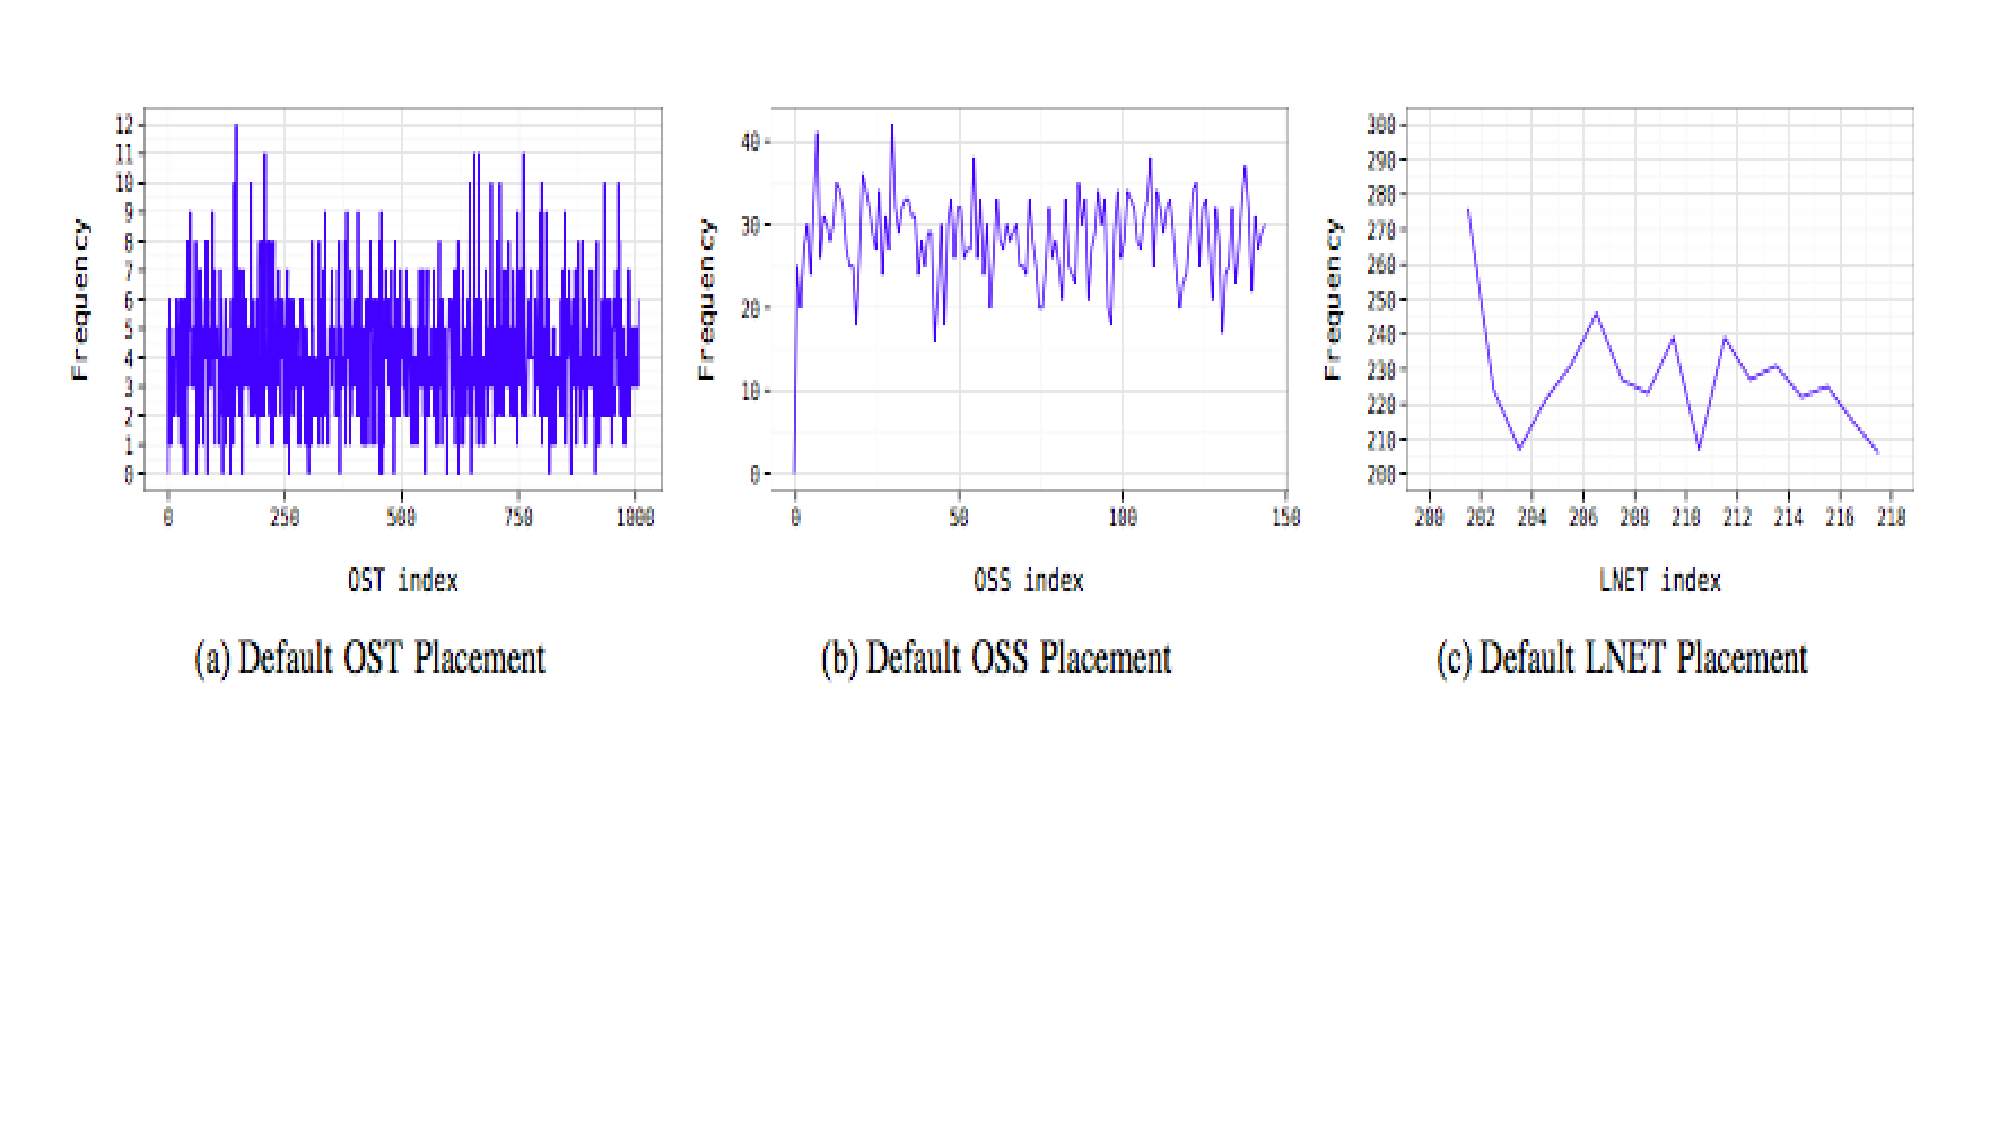
\includegraphics[width=\columnwidth]{graphics/infrastructure.pdf}\vspace{-1.2in}
  \caption{Resource usage distribution for OST(a), OSS(b) and LNETs(c). }
\end{figure}

%%% Local Variables:
%%% mode: latex
%%% TeX-master: "../proposal"
%%% End:



%%% Local Variables:
%%% mode: latex
%%% TeX-master: "../proposal"
%%% End:
